% =====================================================================
% STBV decision-path figure (IEEE-style TikZ, standalone-compilable)
% Corrected: includes B2; fusion label is honest (semantic alarm
% preserved against confident-clean upstream evidence, NOT "conflict
% resolved" -- the DS score is decision-inert on the clean-crypto path;
% the B3 risk band drives the policy floor).
%
% Compile:  pdflatex stbv_decision_path.tex
% Or \input{} the tikzpicture into an IEEEtran figure.
% =====================================================================
\documentclass[tikz,border=6pt]{standalone}
\usepackage{tikz}
\usetikzlibrary{arrows.meta,positioning,shapes.geometric,calc}
\begin{document}
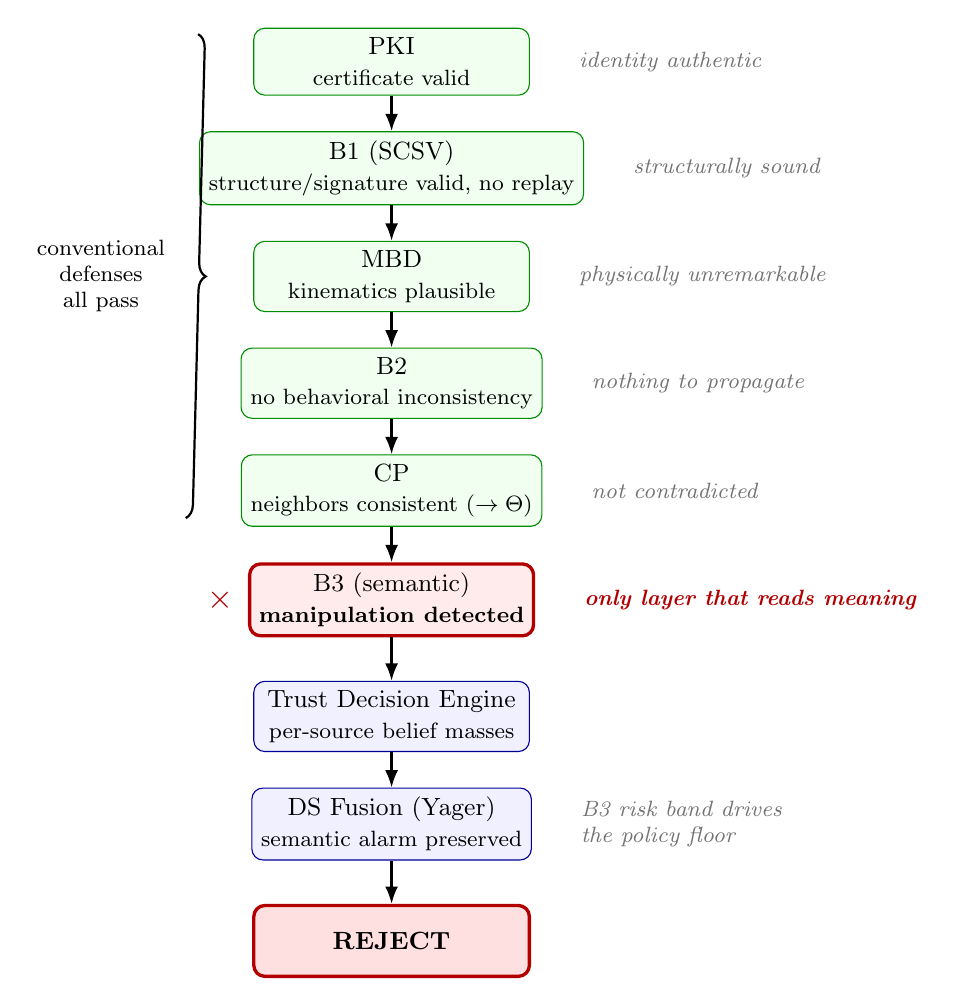
\begin{tikzpicture}[
  font=\small,
  layer/.style={draw, rounded corners, minimum width=3.5cm, minimum height=0.85cm,
                align=center, fill=black!3},
  pass/.style={layer, draw=green!55!black, fill=green!6},
  detect/.style={layer, draw=red!70!black, fill=red!8, very thick},
  engine/.style={layer, draw=blue!60!black, fill=blue!6},
  final/.style={draw, rounded corners, minimum width=3.5cm, minimum height=0.9cm,
                align=center, fill=red!12, draw=red!70!black, very thick},
  arr/.style={-{Latex[length=2.2mm]}, thick},
  note/.style={font=\footnotesize\itshape, text=black!55, align=left, anchor=west},
]
% --- spine ---
\node[pass]   (pki)  {PKI\\ \footnotesize certificate valid};
\node[pass]   (b1)   [below=0.45cm of pki]  {B1 (SCSV)\\ \footnotesize structure/signature valid, no replay};
\node[pass]   (mbd)  [below=0.45cm of b1]   {MBD\\ \footnotesize kinematics plausible};
\node[pass]   (b2)   [below=0.45cm of mbd]  {B2\\ \footnotesize no behavioral inconsistency};
\node[pass]   (cp)   [below=0.45cm of b2]   {CP\\ \footnotesize neighbors consistent ($\rightarrow\Theta$)};
\node[detect] (b3)   [below=0.45cm of cp]   {B3 (semantic)\\ \footnotesize \textbf{manipulation detected}};
\node[engine] (te)   [below=0.55cm of b3]   {Trust Decision Engine\\ \footnotesize per-source belief masses};
\node[engine] (ds)   [below=0.45cm of te]   {DS Fusion (Yager)\\ \footnotesize semantic alarm preserved};
\node[final]  (fin)  [below=0.55cm of ds]   {\textbf{REJECT}};

% --- arrows ---
\foreach \a/\b in {pki/b1,b1/mbd,mbd/b2,b2/cp,cp/b3,b3/te,te/ds,ds/fin}
  \draw[arr] (\a) -- (\b);

% --- checks / cross ---
\foreach \n in {pki,b1,mbd,b2,cp}
  \node[green!55!black] at ($(\n.west)+(-0.35,0)$) {\large\checkmark};
\node[red!70!black] at ($(b3.west)+(-0.35,0)$) {\large$\times$};

% --- right-hand rationale column ---
\node[note] at ($(pki.east)+(0.5,0)$) {identity authentic};
\node[note] at ($(b1.east)+(0.5,0)$)  {structurally sound};
\node[note] at ($(mbd.east)+(0.5,0)$) {physically unremarkable};
\node[note] at ($(b2.east)+(0.5,0)$)  {nothing to propagate};
\node[note] at ($(cp.east)+(0.5,0)$)  {not contradicted};
\node[note, text=red!70!black] at ($(b3.east)+(0.5,0)$)
     {\textbf{only layer that reads meaning}};
\node[note] at ($(ds.east)+(0.5,0)$)
     {B3 risk band drives\\ the policy floor};

% --- STBV annotation brace over the passing layers ---
\draw[decorate,decoration={brace,amplitude=5pt},thick]
     ($(pki.west)+(-0.7,0.35)$) -- ($(cp.west)+(-0.7,-0.35)$)
     node[midway,left=6pt,align=center,font=\footnotesize]
     {conventional\\ defenses\\ all pass};
\end{tikzpicture}
\end{document}